\documentclass[a4paper]{article}
%\usepackage{vntex}
\usepackage{a4wide,amssymb,epsfig,latexsym,multicol,array,hhline,fancyhdr}

\usepackage{amsmath}
\usepackage{lastpage}
\usepackage[lined,boxed,commentsnumbered]{algorithm2e}
\usepackage{enumerate}
\usepackage{color}
\usepackage{graphicx}

% Standard graphics package
\usepackage{array}
\usepackage{tabularx, caption}
\usepackage{multirow}
\usepackage{multicol}
\usepackage{rotating}
\usepackage{graphics}
\usepackage[a4paper,left=2cm,right=2cm,top=1.8cm,bottom=2.8cm]{geometry}
\usepackage{setspace}
\usepackage{epsfig}
\usepackage{tikz}
\usetikzlibrary{arrows,snakes,backgrounds}
\usepackage[unicode]{hyperref}
\hypersetup{urlcolor=blue,linkcolor=black,citecolor=black,colorlinks=true}

\usepackage{float}
%\usepackage{fancyhdr}
\setlength{\headheight}{40pt}
\pagestyle{fancy}
\fancyhead{} % clear all header fields
\fancyhead[L]{
 \begin{tabular}{rl}
    \begin{picture}(25,15)(0,0)
    \put(0,-8){
\includegraphics[width=8mm, height=8mm]{hcmut.png}}
    %\put(0,-8){\epsfig{width=10mm,figure=hcmut.eps}}
   \end{picture}&
	%
\includegraphics[width=8mm, height=8mm]{hcmut.png} & %
	\begin{tabular}{l}
		\textbf{\bf \ttfamily Ho Chi Minh City University of Technology}\\
		\textbf{\bf \ttfamily Department of Computer Science and Engineering}
	\end{tabular}
 \end{tabular}
}
\fancyhead[R]{
	\begin{tabular}{l}
		\tiny \bf \\
		\tiny \bf
	\end{tabular}  }
\fancyfoot{} % clear all footer fields
\fancyfoot[L]{\scriptsize \ttfamily Mathematical Modeling}
\fancyfoot[R]{\scriptsize \ttfamily Page {\thepage}/\pageref{LastPage}}
\renewcommand{\headrulewidth}{0.3pt}
\renewcommand{\footrulewidth}{0.3pt}

%%%
\setcounter{secnumdepth}{4}
\setcounter{tocdepth}{3}
\makeatletter
\newcounter {subsubsubsection}[subsubsection]
\renewcommand\thesubsubsubsection{\thesubsubsection .\@alph\c@subsubsubsection}
\newcommand\subsubsubsection{\@startsection{subsubsubsection}{4}{\z@}%
                                     {-3.25ex\@plus -1ex \@minus -.2ex}%
                                     {1.5ex \@plus .2ex}%
                                     {\normalfont\normalsize\bfseries}}
\newcommand*\l@subsubsubsection{\@dottedtocline{3}{10.0em}{4.1em}}
\newcommand*{\subsubsubsectionmark}[1]{}
\makeatother


\begin{document}

\begin{titlepage}

\begin{center}
VIETNAM NATIONAL UNIVERSITY - HO CHI MINH CITY \\
UNIVERSITY OF TECHNOLOGY \\
DEPARTMENT OF COMPUTER SCIENCE AND ENGINEERING
\end{center}

\vspace{1cm}

\begin{figure}[h!]
\begin{center}

\includegraphics[width=3cm]{hcmut.png}
\end{center}
\end{figure}

\vspace{1cm}


\begin{center}
\begin{tabular}{c}
\multicolumn{1}{l}{\textbf{{\Large MATHEMATICAL MODELING}}}\\
~~\\
\hline
\\
\multicolumn{1}{l}{\textbf{{\Large Assignment}}}\\
\\
\textbf{\Huge Modeling The Coin Selection Problem}\\
\textbf{\Huge In Blockchain Technology}\\
\\
\hline
\end{tabular}
\end{center}

\vspace{4cm}

\begin{table}[h]
\begin{tabular}{rrl}

\hspace{5 cm} & Lecturer: Huynh Tuong Nguyen\\
& CO2011 & CCO1, Group 4\\
& Students: & Vo Dong Ho - 1752219 \\
& & Mai Trong Nhan - 1752390 \\
& & Nguyen Minh Nhat - 1752039 \\
& & Nguyen Minh Quan - 1752450 \\
& & Huynh Gia An Tien - 1752538 \\
& & Pham Minh Tuan - 1752595 \\

\end{tabular}
\end{table}

\begin{center}
{\footnotesize HO CHI MINH CITY, April 2019}
\end{center}
\end{titlepage}

%\thispagestyle{empty}

\clearpage
\tableofcontents
\clearpage

\section{Introduction}
  \subsection{Bitcoin and Blockchain}
  \begin{itemize}
    \item \textbf{Decentralized System}
      \par The idea behind cryptocurrencies is a decentralized system for transactions. Instead of a traditional client-server network, cryptocurrencies like Bitcoin utilize a peer-to-peer network in which every machine on the network, called node, has the same copy of the history of transactions on the network.
    \item \textbf{Blocks and Blockchain}
      \par The history of transactions is stored in a system called \textbf{blockchain}. On this ``chain", each block stores a set of transactions, together with the hash of the previous block. A transaction is said to be confirmed only when a block containing it is put onto the chain.
    \item \textbf{Miners and Transaction Confirmation}
      \par On a network of cryptocurrency, there needs to be some kind of mechanism to confirm transactions by putting them in a new block on the blockchain. The nodes that are responsible for transaction confirmation are called \textbf{miners}.
      \par To be able to create a new block on the blockchain, a miner needs to participate in a race with other miners on the network to find a solution for a ``puzzle". This kind of puzzle is somewhat like lottery tickets. The more computational power a miner has, the higher chance it will be the first one to solve the puzzle - just like the more lottery tickets one buys, the higher chance he or she will win the lottery.
      \par Because the confirmation mechanism is based on computational work, it is super hard for a miner to create a fraudulent transaction, unless it has more than half of the computational power of all miners on the network combined.
      \par After a successful confirmation, a miner will receive bounty from two different sources:
      \begin{itemize}
        \item \textbf{Transaction fee}: each transaction has an amount of transaction fee to attract miners to include it into a new block
        \item \textbf{Coin base}: the network automatically includes an amount of currency called ``coin base" as a prize for the miner.
      \end{itemize}
    \item \textbf{Bitcoin Transactions and UTXOs}
      \par Some cryptocurrencies, such as Bitcoin, use UTXOs (which stands for Unspent Transaction Outputs) as ``inputs" of transactions. We can think of UTXOs as banknotes. When one buys a product in real life, he or she pays with banknotes and then gets an amount of change if the paid amount exceeds the price of the product. It is the same for UTXOs: a transaction takes some UTXOs as inputs, produces some outputs and also a change output if required.
    \item \textbf{Transaction Size and Transaction Fee}
      \par On the current Bitcoin network, an input has a constant size of 148 bits and an output has a constant size of 34 bits. The size of a transaction is the size of all inputs and outputs combined. At a moment, the transaction fee can be computed with the following formula:
      \begin{align*}
        \text{Fee} \approx \text{Fee rate} \times [148 * \text{\# inputs} + 34 * \text{\# outputs}]
      \end{align*}
    \item \textbf{Dust}
      \par Roughly speaking, dust outputs are transaction outputs that are so small that the fee to retrieve it is even larger than the value of itself. The network would try to prevent the creation of this type of outputs by including dust output into the transaction fee.
  \end{itemize}

  \subsection{The Coin Selection Problem}
    \par To understand the Coin Selection problem, we need to understand two objectives:
      \begin{itemize}
        \item Minimizing the transaction fee
        \item Shrinking the UTXO pool
      \end{itemize}

      \subsubsection{Minimizing the Transaction Fee}
        \par Minimizing the transaction fee is what a user wants. In the formula of transaction fee, fee rate is constant at a point in time, and the number of outputs depends on the decision of the user for a particular transaction. What is left is the number of inputs. The larger the number of inputs is, the higher the fee becomes. Therefore, a user would want to use the least number of inputs possible for a transaction.

      \subsubsection{Shrinking the UTXO pool}
        \par It is important to keep the UTXO pool relatively small for performance purpose: the larger the UTXO pool is, the more it hampers processing speed and consumes memory. To shrink the UTXO pool, there are two things we can do:

        \begin{itemize}
          \item Prevent the creation of change output
          \item Select the largest number of inputs possible for one transaction
        \end{itemize}

        \par As we can see, the two objectives somewhat contradict each other: for the previous objective, we want to select as few inputs as possible, while for this objective, we want to do the opposite. Therefore, we always have some kind of trade-off between the two objectives.

        \par Our project try to incorporate these two objectives through two mathematical models solved by linear optimization.

\clearpage


\section{Problem Statement and Modeling}
  \subsection{Problem Statement}
    \par Given a transaction with:
      \begin{itemize}
        \item A set of inputs: each input has a certain value and a size of 148 bits.
        \item A list of outputs: each output has a certain value and a size of 34 bits.
        \item Transaction fee rate
        \item Dust threshold: any output with the value lower than this threshold is considered dust.
      \end{itemize}
    \par Find a way to select inputs such that:
      \begin{itemize}
        \item The transaction size is as low as possible
        \item The number of selected inputs is as large as possible.
      \end{itemize}

  \subsection{Model 1: Minimizing transaction size}
    {
      \small
      \textit{This part is also included as a Jupyter notebook in the source code}
    }

\subsubsection{Problem Modelling}

\begin{itemize}
  \item \textbf{Input parameters}
    \begin{center}
    \begin{tabular}{|c|c|}
    \hline
    \textbf{Variable}                 & \textbf{Meaning}              \\ \hline
    $U = \{u_1, \ldots, u_n\}$        & set of UTXOs                  \\ \hline
    $O = \{o_1, \ldots, o_m\}$        & set of outputs                \\ \hline
    $V^u = \{v_1^u, \ldots, v_n^u \}$ & set of value of UTXOs         \\ \hline
    $V^o = \{v_1^o, \ldots, v_m^o \}$ & set of value of outputs       \\ \hline
    $S^u = \{s_1^u, \ldots, s_n^u \}$ & set of size of UTXOs          \\ \hline
    $S^o = \{s_1^o, \ldots, s_m^o \}$ & set of size of outputs        \\ \hline
    $M_s$                             & maximum size of a transaction \\ \hline
    $\alpha$                          & fee rate                      \\ \hline
    $T$                               & dust threshold                \\ \hline
    $\epsilon$                        & minimum change output         \\ \hline
    \end{tabular}
    \end{center}

  \item \textbf{Decision variables}
  \begin{align*}
    x_i =
    \begin{cases}
    1, \text{if UTXO $u_i$ is chosen} \\
    0, \text{otherwise}
    \end{cases}
  \end{align*}

  \item \textbf{Immediate variables}:
  \begin{itemize}
    \item $y$: transaction size
    \item $z_v$: change output
    \item $z_s$: change value
  \end{itemize}

  \item The relationship between change output value $z_v$ and its size $z_s$:
  \begin{align*}
  z_s =
    \begin{cases}
      0, 0 \leq z_v \leq \epsilon \\
      \beta, z_v > \epsilon
    \end{cases}
  \end{align*}

  \item \textbf{Constraint 1}: A transaction size may not exceed maximum block data size.
  \begin{align*}
y = \sum\limits_{i|u_i \in U} (s_i^u * x_i) + \sum\limits_{j|o_i \in O} s_j^o + z_s \leq M_s
  \end{align*}

  \item \textbf{Constraint 2}: A transaction must have sufficient value for consuming.
  \begin{align*}
\sum\limits_{i|u_i \in U} (v_i^u * x_i) = \sum\limits_{j|o_i \in O} v_j^o + \alpha y + z_v
  \end{align*}

  \item \textbf{Constraint 3}: All the transaction outputs must be higher than the dust threshold to certain that this transaction is relayed to the network and confirmed.
  \begin{align*}
\sum\limits_{j|o_i \in O} v_j^o \geq T
  \end{align*}

  \item \textbf{Objective function}: Minimize transaction size
  \begin{align*}
min(y)
  \end{align*}

\end{itemize}

\subsubsection{Reformulating}

\begin{itemize}
  \item Define $M_c$ as the maximum value of change.
  \begin{align*}
M_{c} = \sum\limits_{i|u_i \in U} (v_i^u * x_i) - \sum\limits_{j|o_i \in O} v_j^o
  \end{align*}

  \item Define a binary variable $t$:
  \begin{align*}
    t =
    \begin{cases}
        0, \text{if $z_v - \epsilon \leq 0$, or if $z_s = 0$}\\
        1, \text{if $z_v - \epsilon > 0$, or if $z_s = \beta$}
    \end{cases}
  \end{align*}

  \item The relationship between $t$ and $z_v$ can be rewritten as a linear inequality:
  \begin{align*}
    z_v - \epsilon \leq M_c t \\
\Rightarrow
    - M_c t + z_v \leq \epsilon
  \end{align*}

  \item Substitute $t$ into $y$:
  \begin{align*}
y = \sum\limits_{i|u_i \in U} (s_i^u * x_i) + \sum\limits_{j|o_i \in O} s_j^o + t \times \beta \leq M_s
  \end{align*}

  \item Substitute $t$ into constraint 1:
  \begin{align*}
    &&\sum\limits_{i|u_i \in U} (v_i^u * x_i)
    &=
    \sum\limits_{j|o_i \in O} v_j^o + \alpha y + z_v \\
&\Rightarrow
    &\sum\limits_{i|u_i \in U} (v_i^u * x_i)
    &=
    \sum\limits_{j|o_i \in O} v_j^o + \alpha \bigg[\sum\limits_{i|u_i \in U} (s_i^u * x_i) + \sum\limits_{j|o_i \in O} s_j^o + t \times \beta\bigg] + z_v \\
&\Rightarrow
    &\sum\limits_{i|u_i \in U} \bigg[\bigg(v_i^u - \alpha s_i^u\bigg) x_i \bigg] - \alpha \beta t - z_v
    &=
    \sum\limits_{j|o_i \in O} v_j^o + \alpha \sum\limits_{j|o_i \in O} s_j^o \\
  \end{align*}

\end{itemize}

\subsubsection{Solving with Linear Optimization}
\par After reformulating, the model can be solved by linear optimization:

Minimize the objective function:
\begin{align*}
  y = \sum\limits_{i|u_i \in U} (s_i^u * x_i) + \sum\limits_{j|o_i \in O} s_j^o + t \times \beta
\end{align*}

subject to the linear constraints:
\begin{align*}
  \sum\limits_{i|u_i \in U} (s_i^u * x_i) + \sum\limits_{j|o_i \in O} s_j^o + t \times \beta \leq M_s
\end{align*}

\begin{align*}
    \sum\limits_{i|u_i \in U} \bigg[\bigg(v_i^u - \alpha s_i^u\bigg) x_i \bigg] - \alpha \beta t - z_v
    =
    \sum\limits_{j|o_i \in O} v_j^o + \alpha \sum\limits_{j|o_i \in O} s_j^o
\end{align*}

\begin{align*}
-M_c t + z_v \leq \epsilon
\end{align*}

and the bounds:

\begin{align*}
    x_i \in \{0, 1\} \forall u_i \in U \\
    t_i \in \{0, 1\} \\
    0 \leq z_v \leq M_c
\end{align*}

  \subsection{Model 2: Maximize the number of selected inputs based on an upper bound of transaction fee}
    {
      \small
      \textit{This part is also included as a Jupyter notebook in the source code}
    }

    \subsubsection{Problem Modelling}
      \par The same with Model 1 with some modifications:
\begin{itemize}
  \item \textbf{Constraint 1}: The size of a transaction cannot exceed the minimum size $Y$ found by Model 1 times $(1 + \gamma)$, where $\gamma \in [0, 1]$ is a choosen coefficient: 
  \begin{align*}
    y = \sum\limits_{i|u_i \in U} (s_i^u * x_i) + \sum\limits_{j|o_i \in O} s_j^o + z_s \leq (1 + \gamma) Y
  \end{align*}

  \item \textbf{Objective function}: Maximize the number of selected UTXOs (and also try to produce no change output)
  \begin{align*}
    \max(\sum\limits_{i|u_i \in U} u_i - t)
  \end{align*}
\end{itemize}


\subsubsection{Solving with Linear Optimization}
After reformulating, the model can be solved by linear optimization:

Minimize the objective function:
\begin{align*}
  \max(\sum\limits_{i|u_i \in U} u_i - t)
\end{align*}

subject to the linear constraints:
\begin{align*}
  \sum\limits_{i|u_i \in U} (s_i^u * x_i) + t \times \beta \leq (1 + \gamma) Y  - \sum\limits_{j|o_i \in O} s_j^o
\end{align*}

\begin{align*}
    \sum\limits_{i|u_i \in U} \bigg[\bigg(v_i^u - \alpha s_i^u\bigg) x_i \bigg] - \alpha \beta t - z_v
    =
    \sum\limits_{j|o_i \in O} v_j^o + \alpha \sum\limits_{j|o_i \in O} s_j^o
\end{align*}

\begin{align*}
  -M_c t + z_v \leq \epsilon
\end{align*}

and the bounds:

\begin{align*}
  x_i \in \{0, 1\} \forall u_i \in U \\
  t_i \in \{0, 1\} \\
  0 \leq z_v \leq M_c
\end{align*}


\section{Implementation and Results}
  \subsection{Coefficient of Model 2}
    \par We produced the result of Model 2 with 4 different values of $\gamma$:
    \begin{itemize}
      \item $10\%$ (\texttt{model2-1})
      \item $25\%$ (\texttt{model2-2})
      \item $40\%$ (\texttt{model2-3})
      \item $50\%$ (\texttt{model2-4})
    \end{itemize}

  \subsection{Programming Language and Library}
    \par The two models mentioned in section 2 are implemented using Python 3. The library that we used to solve Linear Optimization is \href{https://www.mosek.com/}{\texttt{MOSEK}}.

  \subsection{Implementation Issues}
    \par Out of 133 transactions in the dataset, model 1 successfully solved all. Meanwhile, model 2 failed on a few transactions (from 1 to 4 transactions out of 133, according to different values of $\gamma$). The unsolved transactions often have really large number of inputs (more than 19.000). Some transaction was successfully solved with a particular value of $\gamma$ but was unsolved with another value. Based on our observation, as well as the \texttt{MOSEK} documentation, we suspect the unsolved transactions are caused by numerical issues.
    \par To get the full result despite the unsolved transactions of model 2, for each unsolved transaction we will use the result of model 1 instead, since the result of model 1 is one viable solution of model 2.

  \subsection{Results}
    \par The result of the two models is visualized with the following charts.
    \subsubsection{Transaction Size}
      \begin{figure}[H]
        \center{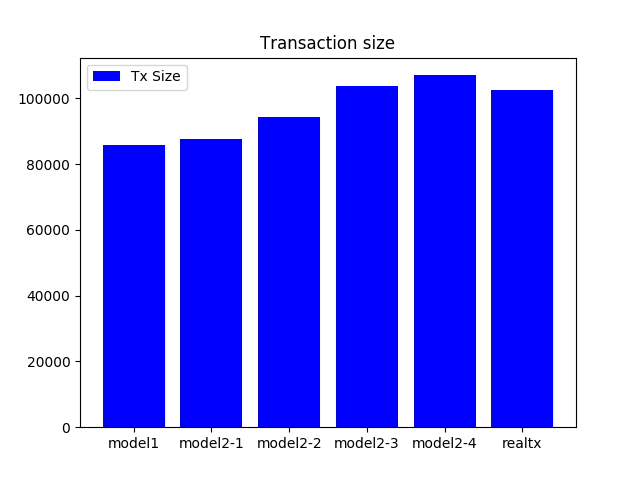
\includegraphics[width=12.5cm]
        {plot01.png}}
      \end{figure}
    \subsubsection{Number of Selected UTXOs}
      \begin{figure}[H]
        \center{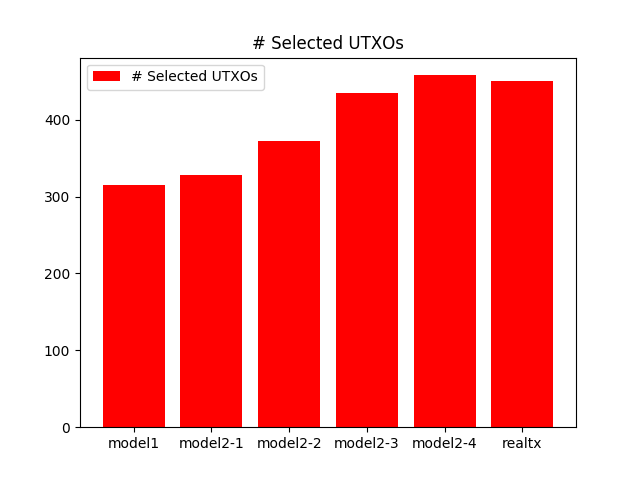
\includegraphics[width=12.5cm]
        {plot02.png}}
      \end{figure}
    \subsubsection{Average Value of Selected UTXOs}
      \begin{figure}[H]
        \center{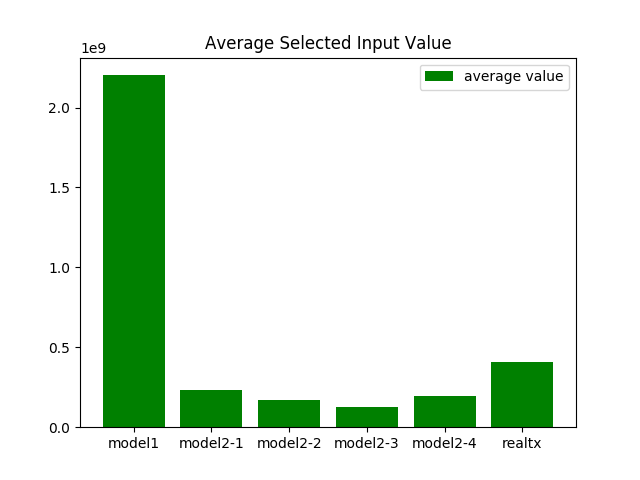
\includegraphics[width=12.5cm]
        {plot03.png}}
      \end{figure}


\end{document}
